\documentclass[russian,11pt]{article}
\usepackage[russian]{babel}
\usepackage[utf8]{inputenc}
% Общие отступы для страницы
\usepackage[left=2cm,right=2cm,
    top=2cm,bottom=2cm,bindingoffset=0cm]{geometry}
% Работа с url
\usepackage{url}
% Работа с изображением
\usepackage{graphicx}
\graphicspath{ {./images/} }
% для листинга
\usepackage{listings}


\begin{document}

\title{Пишем свое первое расширение на Quarkus}
\author{Иванов Роман Александрович}

\maketitle

\newpage
\tableofcontents
\newpage

\section{Предисловие}
~

 Quarkus - это фреймворк, состоящий из ядра и набора расширений. Ядро основано на внедрении Context и Dependency Injection (CDI), а расширения обычно предназначены для интеграции сторонней инфраструктуры путем предоставления их основных компонентов в виде компонентов CDI.

\section{Что такое Quakus Extension}
\paragraph{	} Quarkus Extension- это просто модуль, который может работать поверх приложения Quarkus. Наиболее распространенный вариант использования такого расширения - запуск стороннего фреймворка поверх приложения Quarkus.

\section{Запуск приложения в простом java приложении}
\paragraph{ } 
Давайте попробуем реализовать расширение для отправки почты во время поднятия контекста приложения (будем его дальше называть notification). Но прежде чем мы углубимся, нам сначала нужно показать, как отправлять сообщения из основного метода Java. Это значительно облегчит реализацию расширения. Точкой входа для notification является API notification. Чтобы использовать это, нам нужен адрес отправителя и получателя:

\paragraph{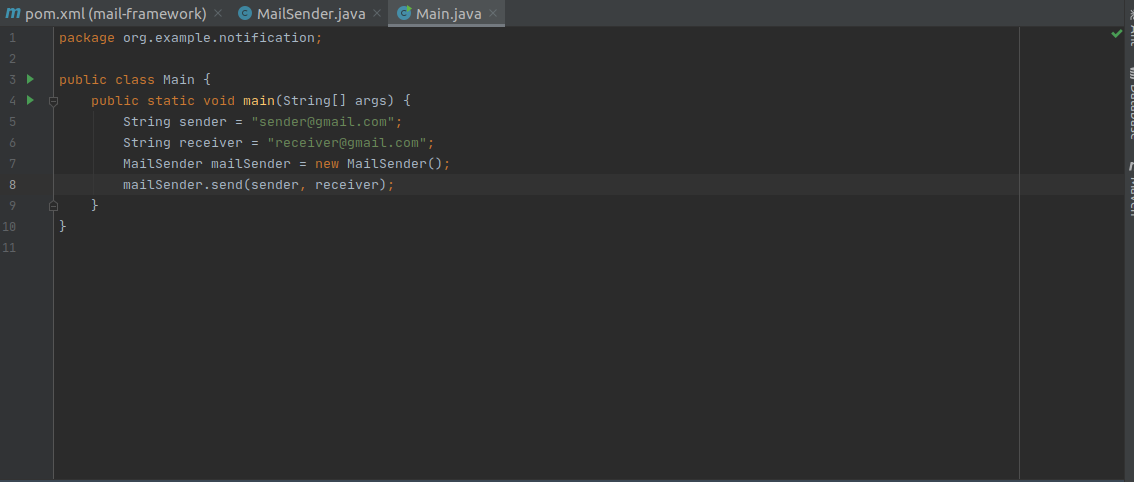
\includegraphics[scale=1.5, width=\textwidth]{1}}
~

При запуске можно увидеть следующее:

\paragraph{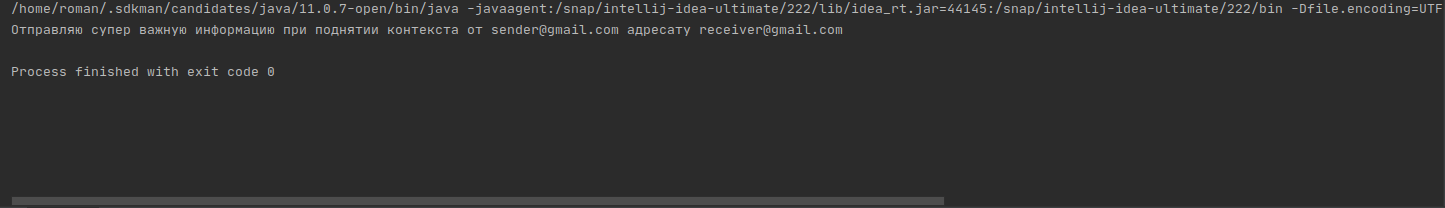
\includegraphics[scale=1.5, width=\textwidth]{2}}

~

Цель состоит в том, чтобы выставить notification как расширение Quarkus. То есть, предоставляя конфигурацию (адрес отправителя и получателя) Quarkus Configuration, а затем создавая notification  API в качестве компонента CDI. Это обеспечит средство для отправки сообщения в момент поднятия контекста приложения.

\section{Как создать расширение}
~

Для ознакомления можно попробовать создать расширение самому, пройдя по ссылке \url{https://quarkus.io/guides/building-my-first-extension}.
	
	Для того, чтобы создать расширение, необходимо выполнить инструкцию:

\lstinputlisting[language=sh]{code/file.sh}

Обратите внимание, что указанная версия 1.4.2.Final является самой актуальной на момент написания, в зависимости от версии ее нужно будет поменять.

	Технически говоря, расширение Quarkus - это многомодульный проект Maven, состоящий из двух модулей. Первый - это модуль времени выполнения, в котором мы реализуем требования. Второй - это модуль развертывания для обработки конфигурации и генерации кода времени выполнения. Итак, начнем с создания многомодульного проекта Maven под названием quarkus-notification-parent, который содержит два подмодуля: время выполнения и развертывание:

\paragraph{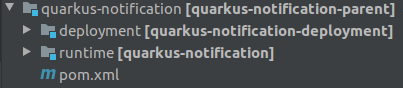
\includegraphics[scale=1, width=\textwidth]{3}}


\section{Имплементация runtime модуля}
\paragraph{ }
В runtime модуле мы реализуем:
 \begin{enumerate}
		\item[  1.] Конфигурационный класс, который будет хранить в себе настройки адресов отправителя и получателя)
		\item[  2.] Поставщика notification API (Предоставление расширением бина, который отвечает за notification API )
		\item[  3.] Рекордер, который будет работать как прокси обьект для вызова API
	\end{enumerate} 
	
	Модуль runtime будет зависеть от модуля ядра Quarkus и, в конечном итоге, модулей времени выполнения необходимых расширений. Здесь нам нужна зависимость нашего импровизированного фреймворка:

\paragraph{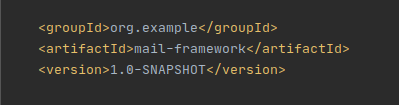
\includegraphics[scale=1.5, width=\textwidth]{4}}


После добавления этой зависимости в runtime модуль он будет выглядеть следующим образом:

\paragraph{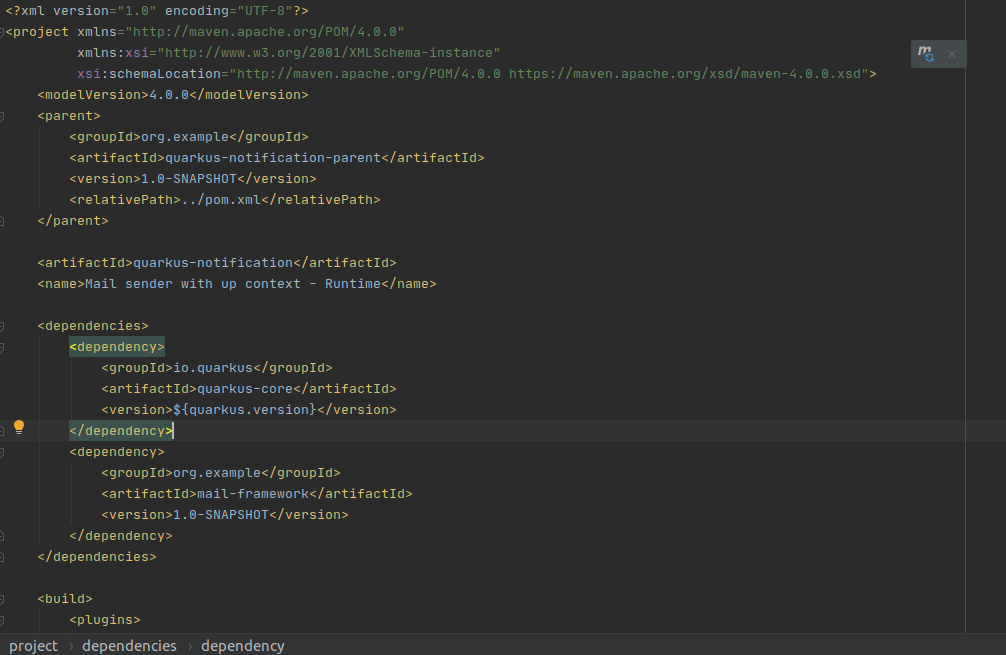
\includegraphics[scale=1.5, width=\textwidth]{5}}

\section{Реализация конфигурации}

Мы аннотируем класс с помощью @ConfigRoot, а свойства - с помощью @ConfigItem. Таким образом, поля from и to, будут представлены через ключ quarkus.mail.from и quarkus.mail.to в файле application.properties, расположенном в пути к классам приложения Quarkus.

	Также стоит обратить внимание на ConfigRoot.phase. Значение  BUILD\_AND\_RUN\_TIME\_FIXED означает, что значения ключей конфигурации читаются во время развертывания и доступен во время выполнения.
	
Конфигурационный класс будет иметь следующий вид:

\paragraph{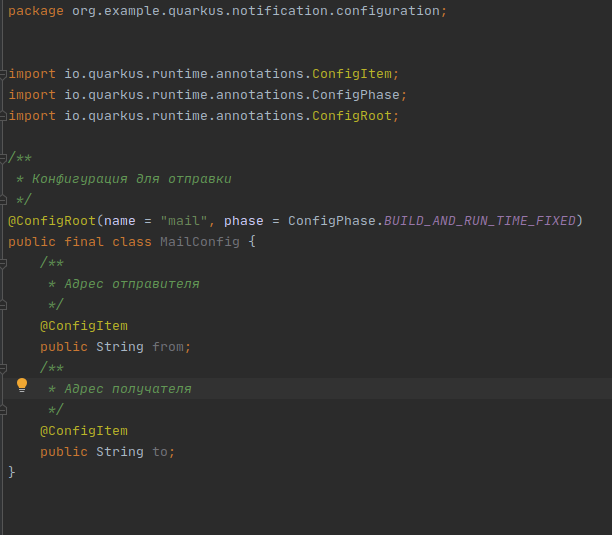
\includegraphics[scale=0.5, width=\textwidth, height=10cm]{6}}

\section{Имплементация поставщика notification API}

Выше мы видели, как работать с notification через простой вызов. Теперь мы воспроизведем тот же код, но в виде компонента CDI, и для этой цели будем использовать производителя CDI:

\paragraph{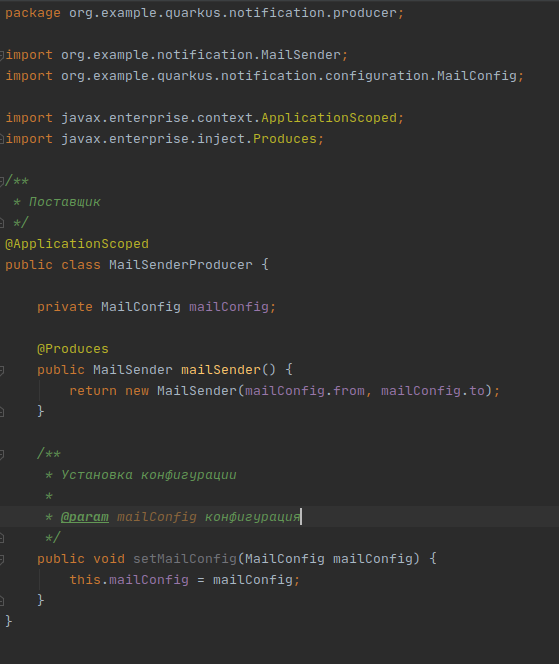
\includegraphics[scale=0.5, width=\textwidth, height=15cm]{7}}
	
	Метод, помеченный аннотацией @Produces, предоставляет бин с настройками, которые будут указаны в application.properties.

\section{Имплементация Рекордера}
~

На этом шаге мы напишем класс Рекордера, который действует как прокси для записи байт-кода и настройки логики времени выполнения:

\paragraph{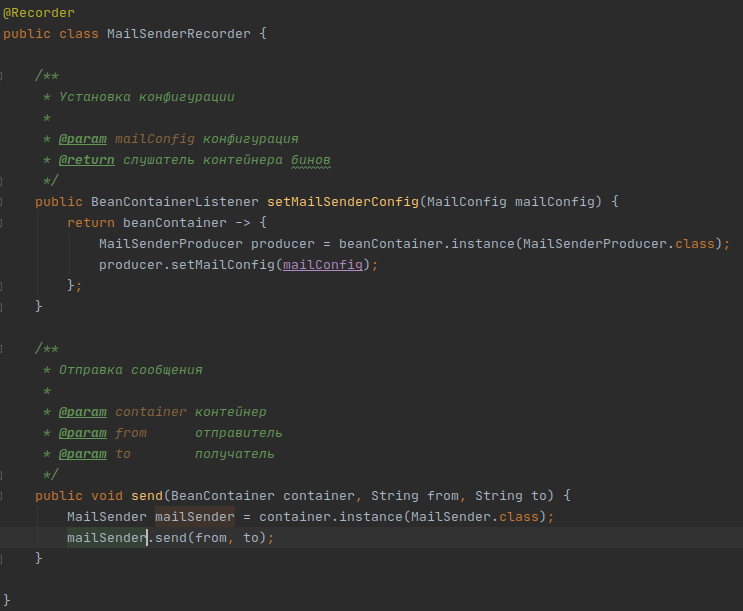
\includegraphics[width=\textwidth, height=18cm]{8}}
~

	Класс рекордер должен содержать аннотацию @Recorder. Через него мы устанавливаем конфигурацию, а также отправляем сообщение.
	
	Обратите внимание, что когда мы вызываем эти методы записи во время сборки, инструкции не выполняются, а записываются для последующего выполнения во время запуска.
	
Далее рассмотрим содержимое модуля развертывания (deployment).

\section{Реализация deployment}

Центральными компонентами расширения Quarkus являются процессоры Build Step. Это методы, аннотированные как @BuildStep, которые генерируют байт-код через устройства записи, и они выполняются во время сборки с помощью цели сборки модуля quarkus-maven-plugin, настроенного в приложении Quarkus.

	BuildSteps потребляют элементы сборки, созданные на ранних этапах сборки, и могут также сами создавать элементы сборки для других этапов сборки.

	Сгенерированный код всеми упорядоченными шагами сборки, найденными в модулях развертывания приложения, фактически является кодом времени выполнения.

\section{Сборка и настройка зависимостей}

Самым важным аспектом зависимостей данного модуля является то, что он должен зависеть от соответствующего модуля времени выполнения и, в конечном итоге, от модулей развертывания необходимых расширений. Это означает, что вам необходимо добавить зависимость runtime модуля в модуль deployment. На нашем примере это выглядит следующим образом:

~

\paragraph{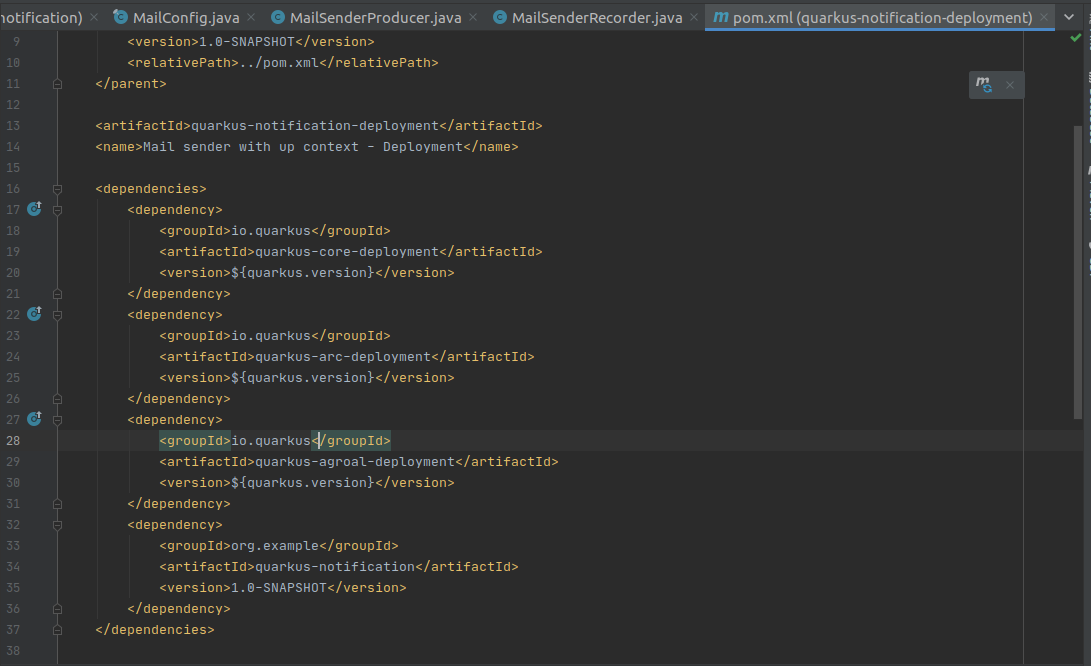
\includegraphics[width=\textwidth, height=18cm]{9}}

\section{Реализация Build Step Processors}
~

Как ранее упоминалось, buildStep это такая инструкция, которая позволяет пошагово настраивать бины и записивать их байткод через инструмент кваркус ARC.

	Теперь давайте реализуем три пошаговых процессора для записи байт-кода. 
Процессором первого шага сборки является метод feature(). Он отвечает за регистрацию расширения в ядро кваркуса.

	За второй шаг сборки отвечает метод build. Он отвечает за регистрацию необходимых BuildItem внутрь других BuildItem. Такой подход позволяет гибко настраивать бины. На этом этапе метод записывает байт-код для выполнения в статическом методе init. Мы настраиваем это через значение STATIC\_INIT, который указан в аннотации @Record.

	Третий шаг сборки описывает метод processSend. Данный метод записывает байт код, который будет выполняться в момент выполнения. Т.е. как только приложение запустится, сразу будет вызван метод отправки сообщения. 


Код процессора выглядит следующим образом:

\paragraph{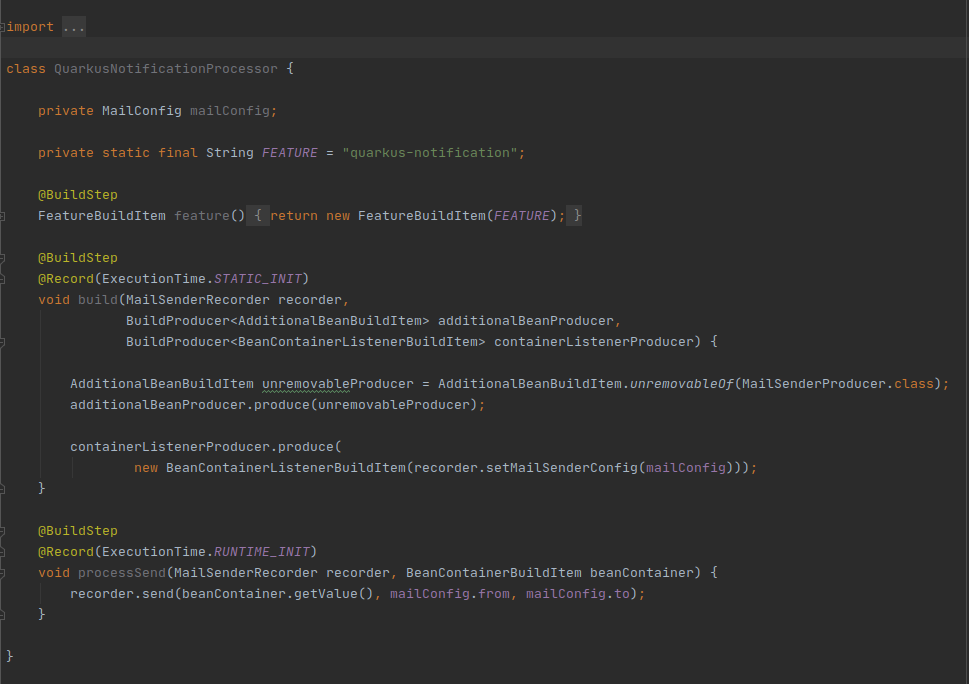
\includegraphics[width=\textwidth, height=10cm]{10}}

\newpage
\section{Тестирование}

Теперь можно протестировать работу расширения. Для этого подключаем ее как зависимость в наш новый проект. Для подключения нужно использовать группу и артефакт от модуля runtime.

\paragraph{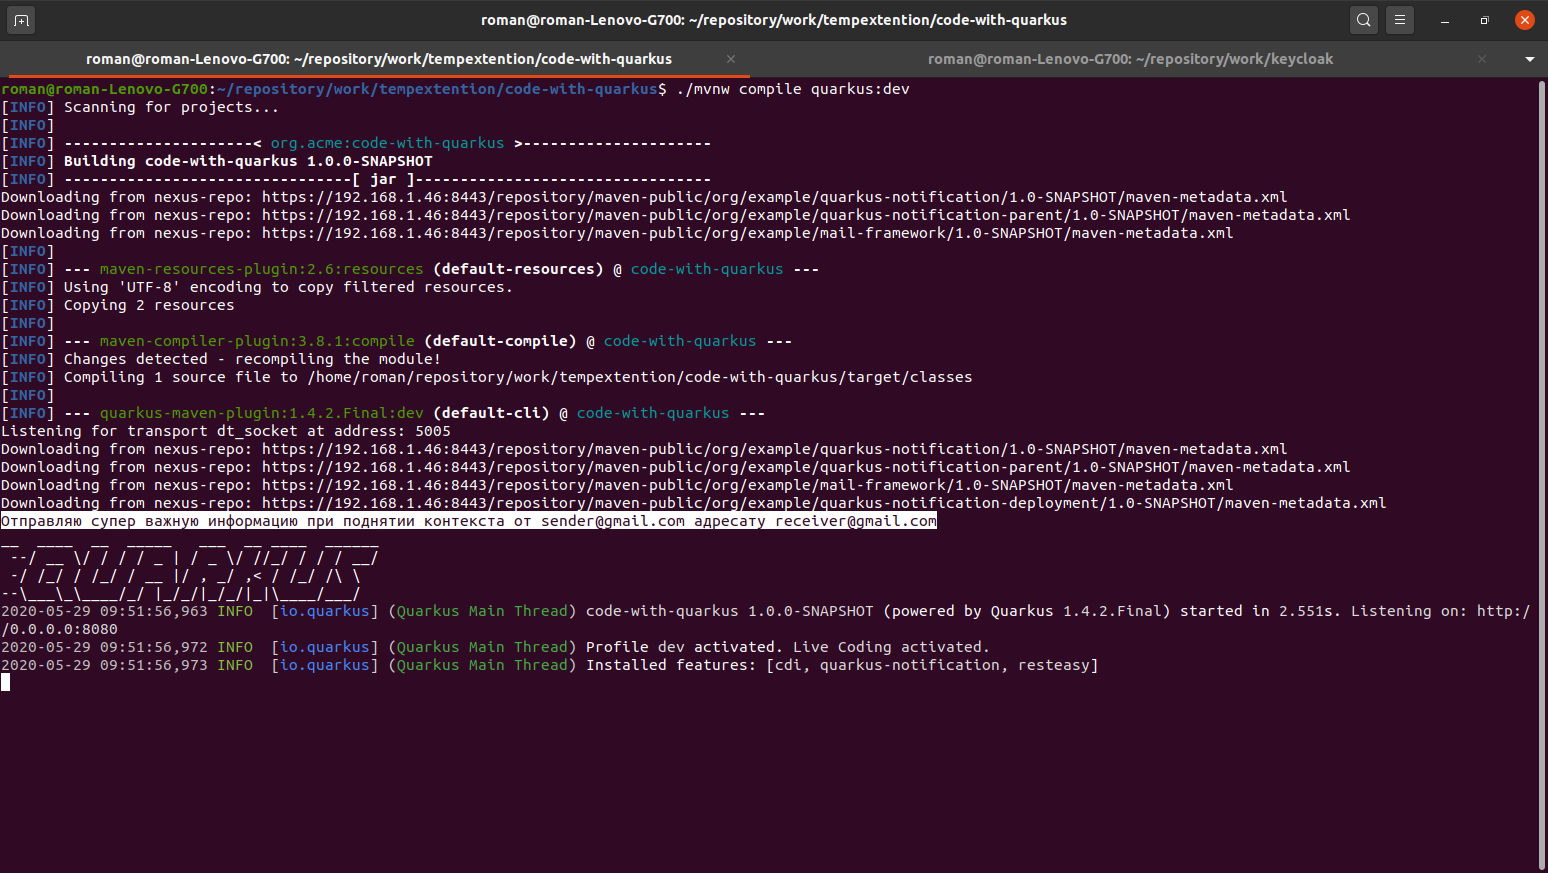
\includegraphics[width=\textwidth, height=18cm]{11}}
~

После запуска мы увидим, что отправляется наше импровизированное сообщение, а также увидим наше расширение в списке подключенных


\end{document}
